\section{绪论}
\zihao{-4}
\setlength{\baselineskip}{20pt}
\fancyhf{}
\renewcommand{\headrulewidth}{0.5pt}
\fancyhead[C]{\zihao{-5}基于MaskedFaceNet的智慧工厂管理系统}
\fancyfoot[C]{\zihao{-5}\tnr\thepage}
\pagenumbering{arabic}

\subsection{研究背景}

随着信息技术的高速发展,越来越多的行业领域开始与这一学科开始交叉挂钩,并且结合出了非常多样的理论知识与应用场景。关于信息管理系统,不管各行各业,无论是高校学籍档案、医疗设备信息还是农业大棚温度测控的场景,都离不开简单高效信息管理系统应用。而且在一些特定的应用场景,不同的信息管理系统所面向的功能也不尽相同,例如有些系统需要面对超大批量用户访问的高并发场景,而有些系统则需要在信息的安全性方面做进一步加强。然而在一些中小型企业工厂的信息管理方式中,例如对工厂员工的信息、客户信息、供应商信息、产品信息以及原材料信息的管理,工厂管理人员大部分往往都是通过手工的方式对信息进行管理,即使人们会用到一些办公软件,例如Word、Excel等;工厂与客户以及供应商的合作方式还都是以电话、微信等联系方式进行沟通交流,但这种方式毫无疑问是离散的、不统一的,并且信息的传递往往都并不是实时的,所以针对中小型工厂企业,设计实现一个通用的、简单易管理的信息管理系统往往有着很大的需求。

人脸识别(Face Recognition)作为一种主流生物识别技术,已经充分的渗透各个领域之中,例如军事、金融、公共安全和日常生活等。并且人脸识别在CVPR(Computer Vision and Pattern Recognition)社区一直是一个火热并且存在长久的研究话题。在上个世纪末,基于特征的人脸识别技术的里程碑出现了,通过特定的分布假设,派生出了一些综合的数学方法对数据的低维表示。直到二十一世纪初,一个众所周知的问题便是这些理论上似乎可信的综合数学方法无法处理的,那就是不可控的面部改变问题。这些问题在\cite{deepfrsurvey}中提到的人脸识别的四个关键时期中,如图\ref{fig:maintime}所示,前三个时期尽管解决人脸识别中的某些面部变化问题,例如姿势变化、光线亮度变化、面部表情和伪装打扮等,但是解决这些问题的方法往往都是比较单一,而且对于识别准确性的提升都是非常有限的。然而这一切都在2012年AlexNet使用了深度学习技术赢下了ImageNet图像分类竞赛的时候发生了巨大的改变。深度学习使用诸如卷积神经网络模型,将多层处理单元进行级联,对输入数据的特征进行提取和变换,从而得到输入数据的多层抽象表示。通过这些多层次的抽象表示,对于人脸姿势、面部表情和光照强度都有着非常强大的不变特性。并且人脸识别技术随着深度学习技术一同飞速发展,直到今天,各种各样的用于人脸识别系统中各个模块的网络模型,都有着超越人类表现的性能。

\begin{figure}
    \centering
    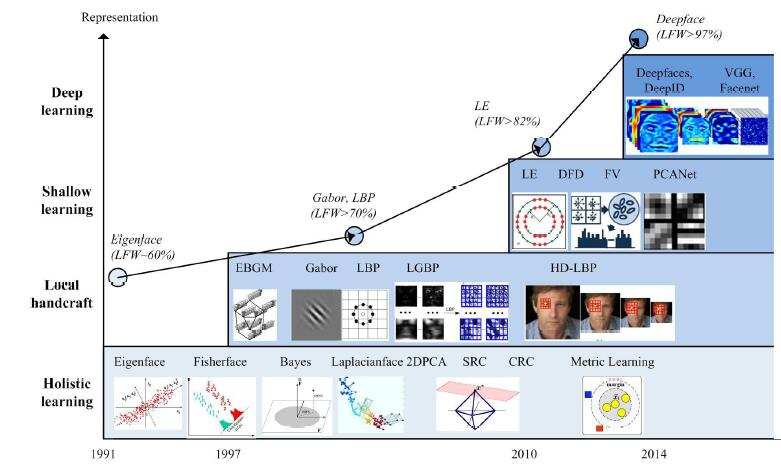
\includegraphics[width=.75\textwidth]{figures/1maintime.jpg}
    \caption{人脸识别技术的四个关键时间点}
    \label{fig:maintime}
\end{figure}

\subsection{国内外研究现状}
